	%------------------------------------------------- Cahier des charges ------------------------------------------------%

	\part{Cahier des charges}
	\parttoc
	
	
	\setcounter{chapter}{0} % Pour recommencer la numérotation des chapitres à 1
	\setcounter{section}{0} % Pour recommencer la numérotation des section à 1
	
	\chapter{Fondements du projet}

		\section{Contexte du projet}
		Le projet proposé est le fruit de la collaboration de l'école polytechnique de l'université de Nantes et de l'entreprise Project2Cloud. Il sera mené de bout en bout par deux étudiants de quatrième année du cycle ingénieur, supervisés par deux professeurs référents. Il s'étendra de septembre à mai. 

		\section{Objectifs du projet}
		L'objectif est de permettre aux étudiants en charge de réaliser un projet professionnel dans le cadre de leurs études. L'objectif du projet est d'ajouter à une plateforme de communication existante un module de transcription textuelle. Chacune des vidéos enregistrées sur la plateforme aura donc un fichier texte associé, qui correspondra à la transcription textuelle de l'audio de cette vidéo. L'intérêt est de rendre plus facile la recherche d'informations à travers les archives vidéos des réunions passées. 

	\chapter{Personnes et organismes impliqués dans le projet}
		\section{Maître d'ouvrage}
		Le maître d'ouvrage sera le contact principal de l'entreprise. C'est avec lui que les étudiants et les tuteurs enseignants seront en relation. Il devra constamment être informé de l'avancement du projet ainsi que des difficultés éventuelles rencontrées. Il pourra interférer à tout moment dans le projet. Son rôle sera de s'assurer que le projet se déroule comme il le désire. Il pourra au besoin demander des modifications ou apporter des précisions sur des points non spécifiés. Toutes les modifications apportées au projet en cours devront être discutées avec les élèves et tuteurs enseignants, pour s'assurer que les objectifs restent adaptés aux contraintes pédagogiques des projets transversaux.  

		\section{Tuteurs enseignants}
		Le rôle des tuteurs enseignant est d'encadrer les étudiants tout au long du projet. Ils devront être tenus informés chaque semaine de l'avancement du projet, ainsi que des difficultés rencontrées. Les tuteurs auront pour rôle de guider les étudiants dans la démarche organisationnelle du projet, et de s'assurer que les objectifs fixés sont respectés à la fin de chaque phase de travail.

		\section{Elèves Étudiants}
		Les deux étudiants seront les concepteurs du projet. C'est à eux de mener de bout en bout le projet. Avec l'aide des tuteurs enseignants et du maître d'ouvrage, ils devront mener à bien le projet, de sa phase de recherche à sa phase de conception. Ils devront rendre compte de leur travail chaque semaine, et respecter les différentes contraintes imposées par le cahier des charges (contraintes temporelles, technologiques...). 

		\section{Utilisateurs du produit}
		Les utilisateurs seront les usagers de la plateforme Project2Cloud. Le projet sera ainsi destiné aux personnes ayant créées un compte sur la plateforme, et désirant rechercher une vidéo. En effet, lors de la recherche vidéo, ce sont les fichiers de transcription associés aux vidéos qui seront utilisés. 


	\chapter{Contraintes sur le projet}

		\section{Contraintes négociables}
			\subsection{Types de modules externes utilisés}	
			L'utilisation de modules et logiciels \bsc{libres} est recommandé. Cette mesure est fonction de la quantité et de la qualité des modules accessibles. Dans le cas où les solutions libres ne correspondraient pas aux attentes du client, l'utilisation de modules propriétaires sera envisagée. Une discussion avec les tuteurs et le maître d'ouvrage devra alors être tenue pour trouver le meilleur compromis technique et financier. 

			\subsection{Environnement de développement du projet}
			\subsubsection{Système d'exploitation}
   			Le projet sera développé pour être utilisé sur une plateforme Linux. 

			\subsubsection{Logiciel et langage de programmation}
			 Le langage informatique utilisé est le langage de programmation orienté objet Java, puisque la plateforme déjà existante est elle même codée avec ce langage. 

			\subsection{Langage reconnu par les modules de transcription}
			Le projet développé sera principalement axé sur la langue française. Le module de transcription devrait donc reconnaître des conversations françaises. Dans le cas où les modules français ne seraient pas suffisamment performant ou indisponibles, une solution de traitement en Anglais pourrait être envisagée. Il conviendrait dans ce cas de discuter avec le maître d'ouvrage et les tuteurs enseignants de la suite à donner au projet. Les recherches d'un module français pourront être abandonnées ou se poursuivre tout au long du projet, dans le cas où un nouveau module serait disponible. 

			\subsection{Fonctionnalités supplémentaires}
			Des fonctionnalités supplémentaires pourront être ajoutées en cours du projet. Ces ajouts éventuels seront fonction de l'avancement du projet, de la validation des fonctionnalités prioritaires. Le choix des fonctionnalités supplémentaires sera discuté avec le maître d'ouvrage et les tuteurs enseignants, pour s'assurer que ces nouveautés restent en accord avec la portée pédagogique du projet transversal. 

		\section{Contraintes non négociables}
			\subsection{Contraintes de temps}				
		Le projet débute après la réunion de lancement qui s'est tenue le 30 septembre 2011, en présence du maître d'ouvrage, des tuteurs et des élèves. Il devra être mené à terme avant le 26 mai 2012. Les étudiants auront à leur disposition une demie-journée par semaine réservée à la mise en œuvre du projet transversal.  
				

		        \subsection{Environnement de fonctionnement du projet}
			La plateforme de communication est actuellement fonctionnelle. Elle est accessible sur internet, via tous les navigateurs web et tous les systèmes d'exploitation(MaC, Windows, Linux). 

			\subsection{Lieu de fonctionnement}
			La plateforme de communication sur laquelle repose le projet est utilisable depuis n'importe quel type d'ordinateur(PC fixe, portable). Par conséquent, et au vue de la mobilité des supports, la plateforme peut être utilisée dans des environnements variés (salle de réunion, lieu public, environnement extérieur...). La contrainte sonore est capitale dans notre projet. Un son ambiant relativement restreint, voir faible est essentiel pour une utilisation optimale du projet.   
	

			\subsection{Contraintes matérielles}
			L'utilisation du produit se fera par l'intermédiaire d'un micro. Il pourra s'agir de différents types de micro (micro intégré à l'ordinateur, micro externe). De la qualité du micro dépendra la qualité de la transcription. En cas de besoin matériel spécifique au projet, l'entreprise devra être en mesure de le fournir. 

			\subsection{Quel est le budget affecté au projet ?}
			Aucun budget spécifique n'est prévu pour ce projet. Il devra être réalisé dans la mesure du possible avec des modules et des logiciels gratuits, ainsi qu'avec le matériel mis à disposition par l'école.  
			
		
                \section{Faits et hypothèses utiles}
			\subsection*{Facteurs influençant le produit, mais qui ne sont pas des contraintes imposées sur les exigences}
			Le facteur le plus influent du projet est la qualité sonore. Elle comprend le niveau sonore ambiant autour de l'utilisateur, la qualité du micro utilisé, la prononciation du locuteur. Tous ces facteurs sont indépendants de la conception, et ne constituent pas d'exigences propres au sujet. 
			
 			\subsection*{Hypothèses que l'équipe fait sur le projet}
			L'équipe considère le projet réalisable. La réussite du projet sera fonction de la bonne communication entre les différents protagonistes.

	\chapter{Exigences fonctionnelles}

		\section{Portée du travail}
			\subsection{La situation actuelle}
			Project2Cloud est une plateforme actuellement en ligne. Elle est accessible à l'adresse : http://project2cloud.org/ . Elle est ouverte aux professionnels et aux particuliers. 
			\begin{figure}[H] 
				\begin{center}
					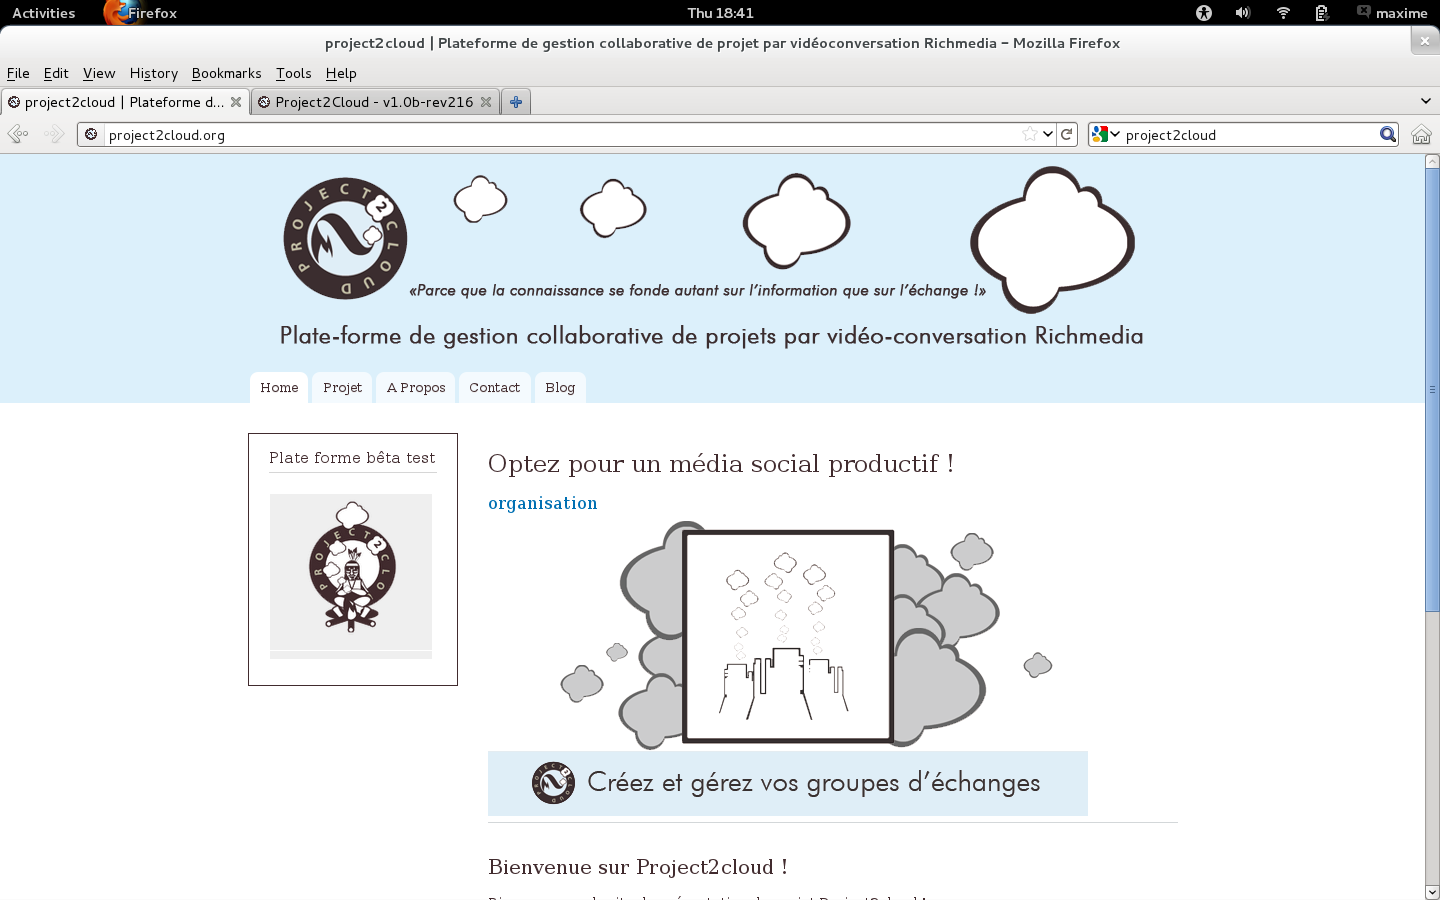
\includegraphics[width=350pt]{site}
					\caption{Site de présentation de l'application.}			
				\end{center}
			\end{figure}

			\begin{figure}[H] 
				\begin{center}
					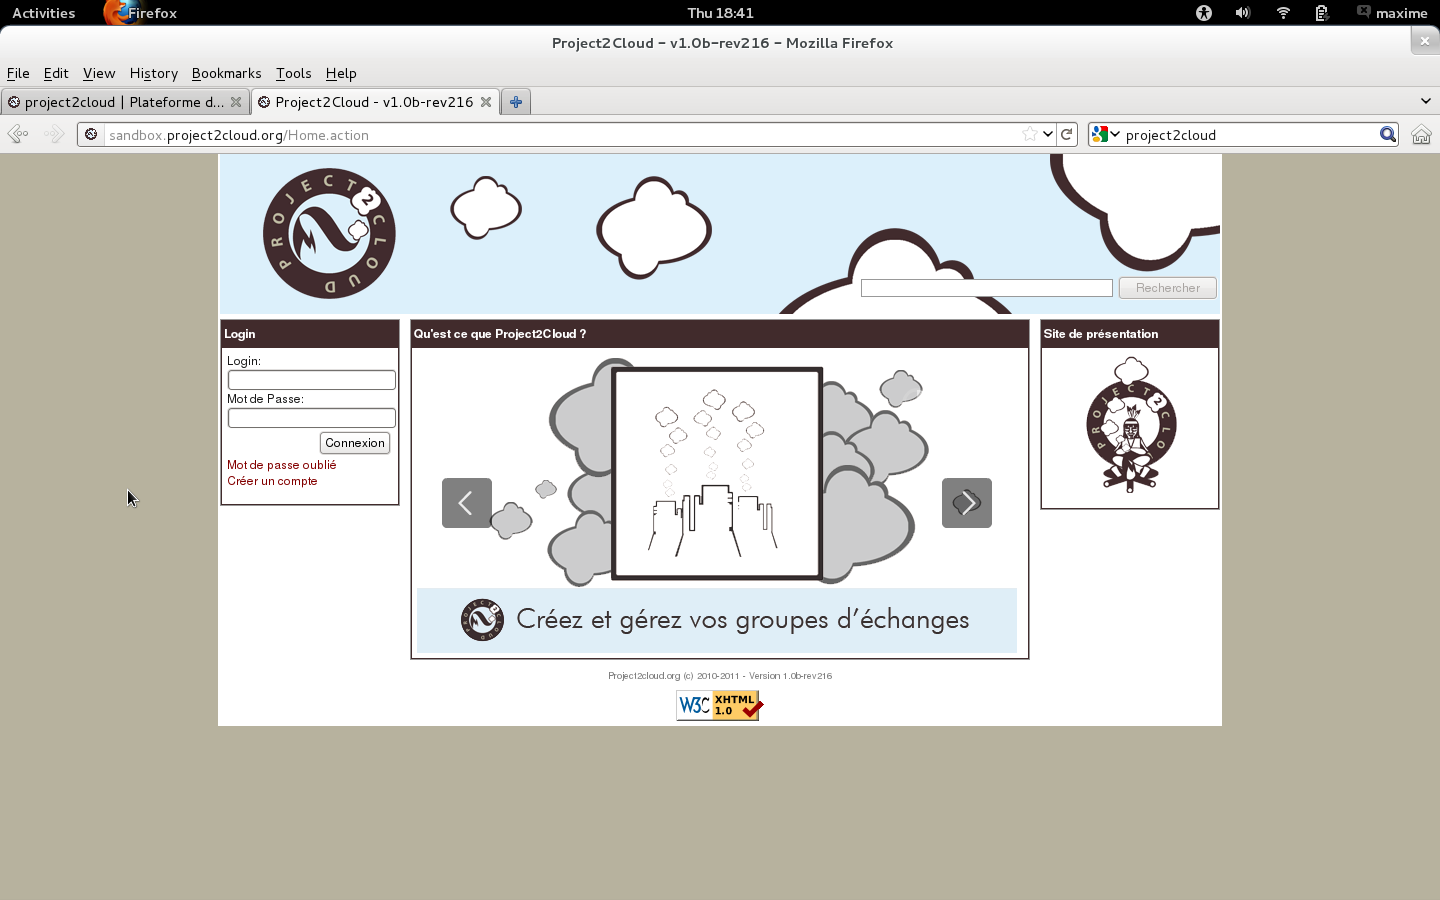
\includegraphics[width=350pt]{plateforme_d_essai}
					\caption{Plateforme Project2Cloud.}			
				\end{center}
			\end{figure}
			
\begin{figure}[H] 
				\begin{center}
					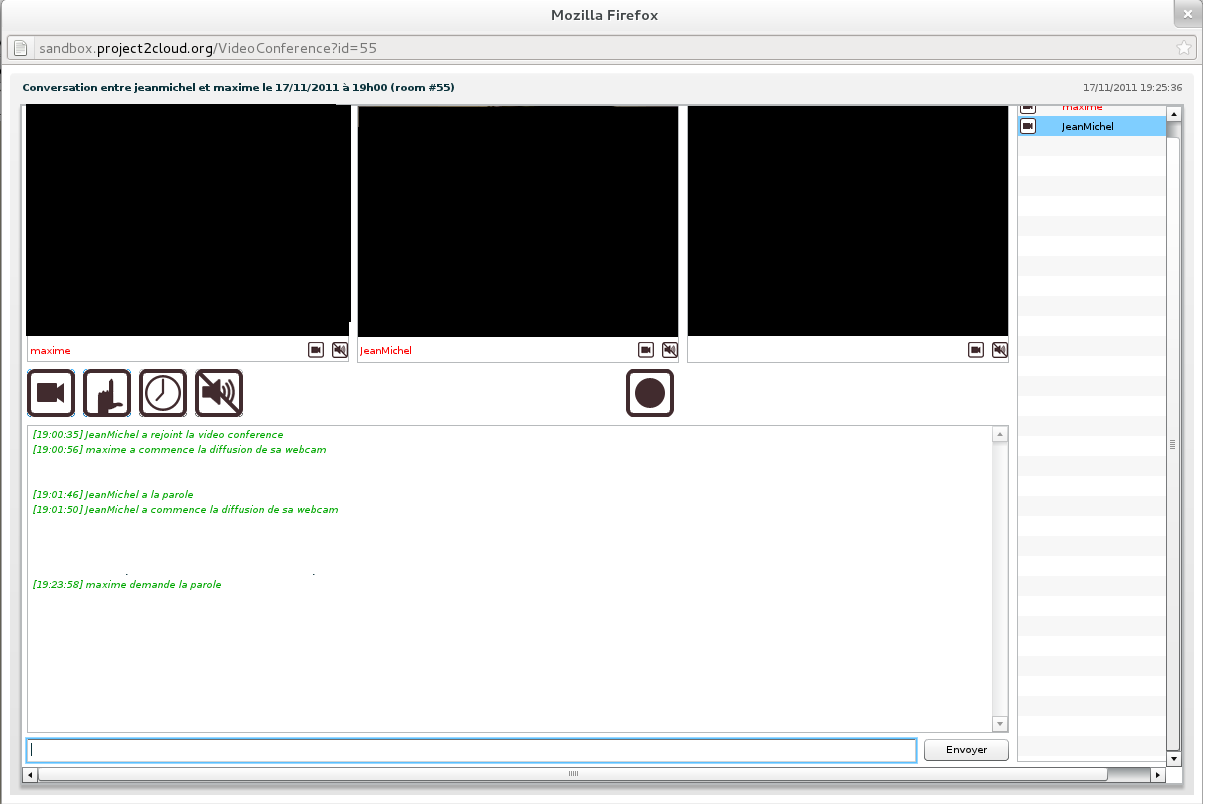
\includegraphics[width=350pt]{videoconf}
					\caption{Conférence vidéo sous Project2Cloud.}			
				\end{center}
			\end{figure}

			\subsection{Contexte du travail}
			Notre projet a pour but d'amener une nouvelle fonctionnalité parmi celles citées précédemment. Celle de retranscrire les conversations des sessions, et ainsi de faciliter l'indexation des conférences vidéos. 

			%\subsection{Division du travail en événements métier}
			
			
			\subsection{Portée du produit (cas d’utilisations)}
			Les cas d'utilisation présentés seront ceux en rapport avec notre projet. Il ne prendront pas en compte les cas d'utilisation de la plateforme déjà existante. Pour la partie transcription de texte, notre module devra recevoir le fichier son encodé par la plateforme et le convertir en fichier texte. Il devra également y associer un fichier XML dans lequel les mots clés de la conversation seront indexés grâce une timeline. Une fois le texte transcrit, ce dernier devra être pris en charge par le serveur. Le serveur devra enregistrer le texte ainsi que l'indexation pour en garder la trace. 

			\begin{figure}[H]
				\begin{center}
					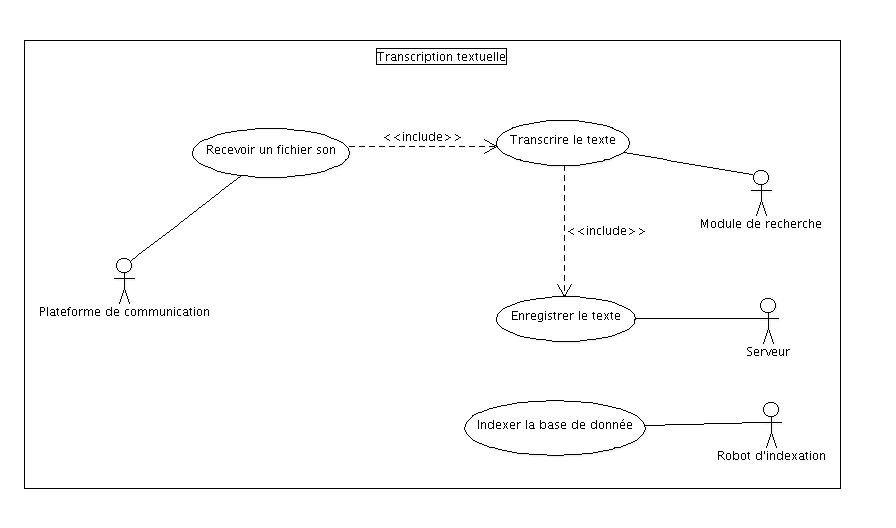
\includegraphics[width=350pt]{UseCaseDiagramTransc}
					\caption{Diagramme des cas d'utilisation de la transcription vocale.}			
				\end{center}
			\end{figure}

			\begin{figure}[H] 
				\begin{center}
					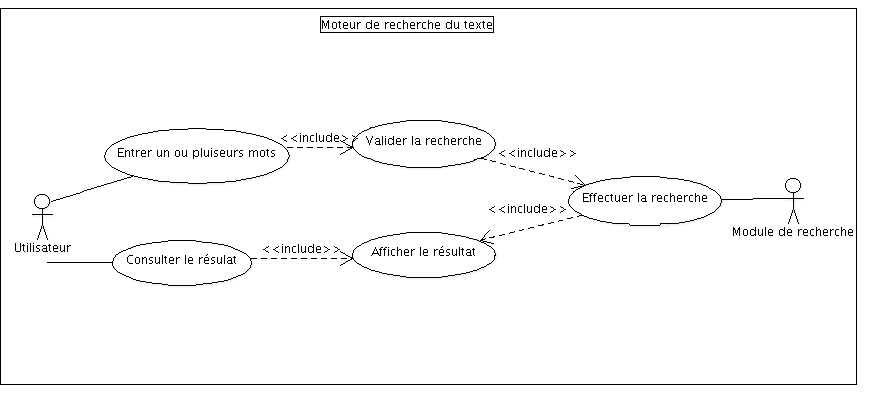
\includegraphics[width=350pt]{UseCaseDiagramMoteur}
					\caption{Diagramme des cas d'utilisation du moteur de recherche.}			
				\end{center}
			\end{figure}

			

			%\subsection{Limites du produit : diagramme de cas d’utilisation}
			

			%\subsection{Description sommaire des cas d’utilisation}
			

		\section{Exigences fonctionnelles et exigences sur les données}

			\subsection{Exigences fonctionnelles}
			Le projet sera basé sur le traitement de fichiers sonores. 
				\subsubsection*{Transcription du fichier son en texte}
				La transcription, ainsi que l'indexation, s'effectueront en tâche de fond. Lors de la réception du fichier son, le module transcrira la voix en texte, et grâce aux modifications apportée, indexera les mots clés dans un second fichier en leur associant leur mappage temporel.
					
				\subsubsection*{Amélioration du modèle de reconnaissance}
				La Plateforme Project2Cloud donnera la possibilité à l'utilisateur d'améliorer manuellement la transcription d'une vidéo. Lorsqu'une telle correction est disponible, le module de recherche peut alors améliorer son modèle de reconnaissance. Lorsque le modèle aura évolué, il sera intéressant de transcrire de nouveau les anciennes vidéos, pour obtenir une meilleure transcription.
				
					
			\subsection{Exigences sur les données}
			Toutes les données mises en jeu dans les modules devront s'adapter avec la plateforme. Elles devront respecter les normes imposées et ne présenter aucun risque de compatibilité. Les formats d'enregistrement et de traitement seront définis plus tard, notamment lors du choix des modules. 
			
		
	
	\chapter{Exigences non fonctionnelles}
			
	
		\subsection{L’interface}
		L'interface sera simple et répondra au mieux aux contraintes imposées. La partie transcription se fait automatiquement, sans intervention de l'utilisateur. Il n'y a donc pas d'interaction avec le client pour cette partie. La partie interrogation, quant à elle, doit être intuitive et facile d'accès pour n'importe quel type d'utilisateur. L'interface n'a pas encore été décidée, elle le sera plus tard, et sera fonction du temps réservé à cette partie du projet. 
	
		\subsection{Le style du produit (packaging inclus)}
		Le produit livré au client n'aura pas de "style" particulier". Les modules seront développés indépendamment de la plateforme, et y seront rattaché en fin de projet. Il n'est donc pas nécessaire d'inclure une notion de style dans notre projet.
	
	
	\section{Facilité d’utilisation et facteurs humains}
		\subsection{Facilité d’utilisation}
		La partie transcription ne sera pas visible pas l'utilisateur. Il interagira avec la plateforme Project2Cloud comme il le ferait actuellement, puisque la transcription se fera automatiquement, sans aucune intervention de sa part. La facilité d'utilisation de cette partie de notre projet est donc fonction de la facilité d'utilisation actuelle. 
		 
	
		\subsection{Personnalisation et internationalisation}
		Le module ajouté à la plateforme ne sera pas personnalisable par l'utilisateur. L'interface et les fonctionnalités mis en place sur la plateforme ne pourront pas être modifiés. 	
		La langue de base de la plateforme est le français. Le site internet est entièrement rédigé en français et ne propose pour le moment pas d'autre langue. Le projet à pour but de ne reconnaitre que des voix françaises, sans proposer d'alternative dans d'autres langues. Il n'y a donc pas de projet d'internationalisation pour le moment. 
	 
	
	
		\subsection{Exigences d’accessibilité}
		Le projet étant intégré dans une plateforme déjà existante, les exigences d'accessibilité seront les même qu'actuellement.
	
	
	\section{Fonctionnement du produit}
		\subsection{Rapidité d’exécution et temps de latence}
		La transcription n'a pas besoin d'avoir un temps d'exécution rapide puisqu'elle se fera automatiquement sur un serveur. 

		
		\subsection{Précision et exactitude}
		La transcription se devra d'être la plus précise possible. Le degrés de précision dépendra cependant de la qualité du module sélectionné.   Éventuellement, plusieurs possibilités de transcriptions pourront être sauvegardées. Le moteur d'interrogation devra prendre en compte que les transcriptions ne sont pas toujours correctes, et donc faire une recherche avec des mots phonétiquement proches.
	
		\subsection{Fiabilité et disponibilité}
		Le projet devra être entièrement fiable et répondre au mieux à la demande du client. La qualité de la transcription ne sera pas en rapport avec le bon fonctionnement du module. Aucune erreur grave ne devra survenir pendant la transcription, sous peine de perdre complètement l'intérêt du projet. La partie recherche devra elle aussi être fiable et sans aucune erreur fatale. 
	
		\subsection{Robustesse ou tolérance à un emploi erroné}
		La qualité de la transcription dépendra du module sélectionné mais également de la qualité de parole de l'utilisateur. Une locution claire et articulée est conseillée pour un résultat optimal. Dans le cas d'une locution médiocre ou d'une mauvaise qualité du son d'entrée, les résultats seront erronés et ne peuvent pas être connus à l'avance. 
		Pour la partie recherche, le module prendra en compte toutes les erreurs potentielles que pourrait commettre l'utilisateur (saisie d'un mot inexistant, validation de la recherche sans mot écrit dans la zone de recherche...). Le module interagira dans ce cas avec l'utilisateur pour lui indiquer la nature de son impair. 
 
		\subsection{Capacité de stockage et montée en charge}
		A ce stade du projet, nous ne connaissons pas encore les capacités limites de stockage et la montée en charge du projet. 
	
		\subsection{Adaptation du produit à une augmentation de volume à traiter}
		Le projet devra pouvoir gérer une augmentation de volume d'utilisateurs. Quelque soit le nombre d'utilisateurs connectés simultanément, le module devra être en mesure d'offrir la même qualité de service à tous.  
	
		\subsection{Longévité}
		Le projet devra être opérationnel sur la durée que le client jugera nécessaire. C'est à lui que reviendra le choix de la longévité du produit. Les modules développés devront aussi être adaptables dans le temps, pour une éventuelle amélioration future. La longévité du projet déprendra donc aussi de sa qualité de réutilisation (code source commenté, documentation explicite et complète...).
	
	\section{Adéquation du produit avec son environnement}
		\subsection{Environnement physique prévu}
		Le projet sera intégré directement dans une plateforme existante. Il devra donc parfaitement s'intégrer avec le site internet hôte.
	
		\subsection{Environnement technologique prévu}	
		L'environnement technologique sera uniquement le web. 
	
		\subsection{Applications « partenaires » (avec lesquelles le produit doit collaborer)}
		Le projet n'a pas pour but de collaborer avec des applications autres que la plateforme hote qui le reçoit. 
	
		\subsection{Approche « produit » prêt à être commercialisé}
	
	
	\section{Maintenance, support, portabilité, installation du produit}
		\subsection{Maintenance du produit}
		Une fois le produit livré et validé par le client, la maintenance ne sera plus assurée dans le cadre du projet transversal. 
	
		\subsection{Conditions spéciales concernant la maintenance du produit}
		Aucune condition spéciale concernant la maintenant n'est à définir dans le cadre du projet. 
	
		%\subsection{Exigences en matière de support}
	
		%\subsection{Exigences de portabilité}
	
		\subsection{Installation du système}
		A ce stade du projet, nous ne sommes pas en mesure de répondre à cette section du cahier des charges. 
	
	
	\section{Sécurité}
		\subsection{Accès au système}
		A ce stade du projet, nous ne sommes pas en mesure de répondre à cette section du cahier des charges. 	

		\subsection{Intégrité}
		A ce stade du projet, nous ne sommes pas en mesure de répondre à cette section du cahier des charges. 

		\subsection{Protection des données à caractère personnel}
		Les données à caractère personnel ne sont pas directement liée à notre projet. Ces données sont gérées par la plateforme en place. 
	
		\subsection{Audit et traçabilité}
A ce stade du projet, nous ne sommes pas en mesure de répondre à cette section du cahier des charges. 
	
		\subsection{Protection contre les infections}
		A ce stade du projet, nous ne sommes pas en mesure de répondre à cette section du cahier des charges. 
	
	
	\section{Exigences culturelles et politiques}
		\subsection{Exigences culturelles}
		Aucune exigence culturelle n'est spécifiée pour ce projet.
	
		\subsection{Exigence politiques}
		Aucune exigence politique n'est spécifiée pour ce projet.
	
	
	\section{Lois et standards influençant le produit}
		\subsection{Conformité avec la loi}
		Le projet sera conforme avec la loi et les exigences juridiques française. 
	
		\subsection{Conformité avec des standards}
		A ce stade du projet, nous ne sommes pas en mesure de répondre à cette section du cahier des charges. 

	\chapter{Autres aspects du projet}
		\section{Questions sans réponse}
		
		\section{« COTS » : Progiciels ou composants commerciaux}
		A ce stade du projet, nous ne sommes pas en mesure de répondre à cette section du cahier des charges. 

		\section{Nouveaux problèmes, créés par l’apparition du nouveau système}
		A ce stade du projet, nous ne sommes pas en mesure de répondre à cette section du cahier des charges. 

		\section{Tâches à faire pour livrer le système}
		A ce stade du projet, nous ne sommes pas en mesure de répondre à cette section du cahier des charges. 

		\section{Contrôle final de qualité sur site (Cutover)}
		A ce stade du projet, nous ne sommes pas en mesure de répondre à cette section du cahier des charges. 

		\section{Risques liés au projet}
		Les risques éventuels liés au projet seront découverts au moment de la partie de conception, et dépendront du langage informatique utilisé. 

		\section{Estimation des coûts du projet}
		Le projet n'aura aucun coût spécifique. 

		\section{Manuel utilisateur et formations}
		Les manuels utilisateurs et formations seront conçus au fur et à mesure de l'avancement du projet. 

		\section{Salle d’attente : idées pour les futures versions}
		Les idées pour des versions futures n'ont pas été abordées. Elles le seront dans le cas où l'avancement du projet le permettrait, et résulteraient d'un accord entre les tuteurs enseignants et le maître d'ouvrage.